\documentclass[11pt,titlepage,contentspage,a4paper]{article} %padrao letterpaper, 10pt
\usepackage[utf8]{inputenc}
\usepackage[portuguese]{babel}
\usepackage{amsfonts,amssymb,graphicx,enumerate}
\usepackage[centertags]{amsmath}
\usepackage[hmargin=2cm,vmargin=3.5cm,bmargin=3cm]{geometry}
\usepackage{fancyvrb}
\usepackage{fancyhdr}% logo para cabecalhos
\usepackage{graphicx}
\usepackage{eso-pic} % marca de água para logos
\renewcommand{\headheight}{0.6in}
\setlength{\headwidth}{\textwidth}
\fancyhead[L]{}% empty left
\fancyhead[L]{ % right
   
\includegraphics[height=0.53in]{logo-ee.jpg}}
\pagestyle{fancy}
\setlength{\unitlength}{1mm}
\newcommand\BackgroundPic[3]{
\put(#2,#3){\parbox[b][\paperheight]{\paperwidth}{
\vfill
\centering
\includegraphics{#1}
\vfill
}}}

\parindent=0pt
\parskip=2pt






\begin{document}
%--- Logo Capa ---%
\AddToShipoutPicture*{\BackgroundPic{logo_eeng.jpg}{-230}{360}}




\title{Modelos Determinísticos de Investigação Operacional \\ 
\begin{large} 
	Trabalho 1 - Grupo 19 
\end{large}}
\author{\begin{small}
William Sousa 61029; Jose Gonçalves 58657; João Carlos 53690; Axel Silva 53064; Andreia Alves 54759.\end{small}}
\date{\today}



\maketitle

\tableofcontents %Índice de conteúdos

\newpage

\section{Introdução}
Este relatório tem como objetivo a análise do primeiro trabalho da unidade curricular  Modelos Determinísticos de Investigação Operacional.
Neste trabalho, foi apresentado o problema do caminho mais longo, também conhecido como caminho crítico, tendo como contexto as tarefas necessárias para a conclusão de um projeto fictício, o qual vai ser o caso de estudo. As tarefas do projeto têm relações de precedência e durações determinísticas conhecidas, formando, assim, um grafo acíclico dirigido, que é uma das bases para todos os modelos aqui apresentados.
Numa primeira parte, iremos modelar e procurar uma solução para o problema apresentado, tirando partido do princípio de conservação de fluxo. No entanto, esta solução apenas fornece informação acerca do caminho crítico.
Numa segunda parte, trataremos o problema, tirando proveito da noção de precedência temporal entre as atividades e formando, assim, um modelo mais robusto que permite apurar e acomodar outros tipos de restrições, tais como o custo associado a cada atividade e uma possível redução no tempo de atividades específicas.
Por fim, procuraremos modelar o sistema de forma correta e precisa. Esta tarefa poderá ser útil tanto para aprofundar conhecimentos ao nível operacional das ferramentas, nomeadamente do LPSolve, como ao nível científico, permitindo-nos adquirir maior sensibilidade acerca das dificuldades associadas à modelação de sistemas complexos em modelos de programação linear.
%%%%%%%%%%%%%%%%%%%%%%%%%%%%%%%%%%%%%%%%%%%%%%%%%%%%%%%%%%%%%%
\section{Parte I}
%%%%%%%%%%%%%%%%%%%%%%%%%%%%%%%%%%%%%%%%%%%%%%%%%%%%%%%%%%%%%%
\subsection{Questão 1}
A rede correspondente à remoção das tarefas 2 e 9 do projeto é a seguinte:
\begin{center}
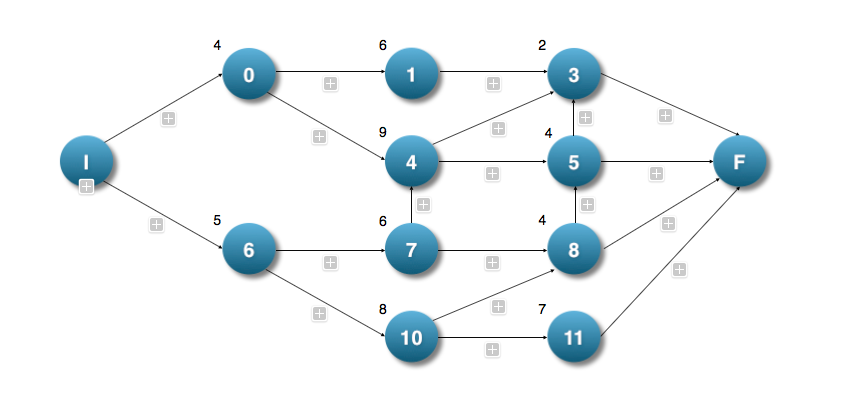
\includegraphics[width=\textwidth]{grafo}
\end{center}

\subsection{Questão 2}
O objetivo deste exercício é a determinação de um modelo em programação linear que estipule o caminho mais longo, ou caminho crítico, da rede de um projeto. Seguindo o enunciado, as variáveis de decisão para este modelo serão descritas da forma $X_{[origem ] [destino]}$, cada uma associada a um arco do grafo. Cada arco assume o valor 1 unidade de fluxo, caso faça parte do caminho crítico, ou o valor 0, caso contrário.

A função objetivo é constituída pelo somatório de todos os arcos (i.e. as variáveis de decisão), cada um multiplicado pela duração associada ao nodo de origem do arco. Uma vez que estamos à procura de um extremo condicional e queremos o caminho mais longo do projeto, optamos por um máximo, resultando na seguinte função objetivo:
\begin{Verbatim}[frame=single]
max: 4x01+4x04+6x13+2x3f+9x43+9x45+4x53+4x5f+5x67+5x610+6x78+6x74+
4x85+4x8f+8x108+8x1011+7x11f;
\end{Verbatim}
Na determinação das restrições, foi seguido o princípio da conservação de fluxo num grafo acíclico dirigido. Começando por injetar uma unidade de fluxo no nodo "início", ação essa representada na restrição $x_{i0}+x_{i6}=1; $ as seguintes restrições obrigam a que o fluxo em todos os nodos seja igual a zero. Salientamos que mantivemos a última restrição, que indica a saída de uma unidade de fluxo do grafo, uma vez que não só se tratava de um problema académico com dimensões e um número de restrições computacionalmente simples, mas também permitiria manter a coerência sobre a preservação do fluxo. No entanto, mesmo que essa restrição tivesse sido eliminada, não alteraria o modelo, pois não haveria outro caminho possível para que a unidade de fluxo pudesse prosseguir após ter passado pelos nodos que representam o fim do projeto.
  

\subsection{Questão 3}
Input utilizado no LPSolve:
\begin{Verbatim}[frame=single]
/* Objective function */
max:4x01+4x04+6x13+2x3f+9x43+9x45+4x53+4x5f+5x67+5x610+6x78+
6x74+4x85+4x8f+8x108+8x1011+7x11f;

/* Restrictions - Princípio da conservação de fluxo */

//início do fluxo
xi0+xi6=1;

//conservação do fluxo
-xi0+x01+x04=0; // nodo 0
-x01+x13=0; // nodo 1
-x13-x43-x53+x3f=0 ;// nodo 3
-x04-x74+x43+x45=0; // nodo 4
-x45-x85+x53+x5f=0; // nodo 5
-xi6+x67+x610=0; // nodo 6
-x67+x74+x78=0; // nodo 7
-x78-x108+x85+x8f=0;// nodo 8
-x610+x108+x1011=0; // nodo 10
-x1011+x11f=0; // nodo 11

// fim do fluxo
-x3f-x5f-x8f-x11f=-1;

\end{Verbatim}
\subsection{Questão 4}
Output do LPSolve:
\begin{Verbatim}[frame=single]
Variables	result
		  26
x01		0
x04		0
x13		0
x3f		1
x43		0
x45		1
x53		1
x5f		0
x67		1
x610	       0
x78		0
x74		1
x85		0
x8f		0
x108	       0
x1011	      0
x11f	       0
xi0		0
xi6		1
\end{Verbatim}

\subsection{Questão 5}
A rede abaixo representa o caminho crítico (i.e. os nodos preenchidos com a cor laranja), que consiste no caminho formado pelas tarefas 1, 6, 7, 4, 5 e 3.

\begin{center}
\includegraphics[width=\textwidth]{grafocritico}
\end{center}

 
%%%%%%%%%%%%%%%%%%%%%%%%%%%%%%%%%%%%%%%%%%%%%%%%%%%%%%%%%%%%%%
\section{Parte II}
%%%%%%%%%%%%%%%%%%%%%%%%%%%%%%%%%%%%%%%%%%%%%%%%%%%%%%%%%%%%%%
\subsection{Questão 1}

Para esta segunda parte, pretendeu-se encontrar o tempo mínimo de execução total do projeto, através de um modelo em programação linear. As variáveis de decisão são descritas como $t_{[atividade]}$ e representam o tempo de início da atividade a que se referem.  

A função objetiva é trivial, pois apenas constitui a variável $t_f$, que representa o tempo de início da atividade do nodo “fim”, ou seja, a duração total do projeto, que deve ser minimizada:	
\begin{Verbatim}[frame=single]
min:tf;
\end{Verbatim}
				
As restrições do modelo devem especificar as precedências temporais a que o projeto está sujeito. Assim, o tempo de início de uma dada atividade deverá ser maior ou igual do que a soma da duração da atividade anterior com o tempo de início desta. Deste modo, uma atividade que tenha uma precedência só pode iniciar no momento em que a anterior termina. Aplicando essas restrições a todas as tarefas e às suas respetivas precedências, o modelo fica formulado.


\subsection{Questão 2}
Input utilizado no LPSolve:
\begin{Verbatim}[frame=single]
/* Objective function */
min:tf;

//* Restrictions - Precedências Temporais */
t0>=0;
t1>=4+t0;
t3>=6+t1;
t3>=9+t4;
t3>=4+t5;
t4>=4+t0;
t4>=6+t7;
t5>=9+t4;
t5>=4+t8;
t6>=0;
t7>=5+t6;
t8>=6+t7;
t8>=8+t10;
t10>=5+t6;
t11>=8+t10;
tf>=2+t3;
tf>=4+t5;
tf>=4+t8;
tf>=7+t11;
\end{Verbatim}


\subsection{Questão 3}
Ouput do LPSolve:
\begin{Verbatim}[frame=single]
Variables	result
		  26
tf		26
t0		 0
t1		 4
t3		24
t4		11
t5		20
t7		 5
t8		13
t6		 0
t10		5
t11	       13
\end{Verbatim}


\subsection{Questão 4}
No seguinte diagrama de Gantt é possível analisar o comportamento do projeto face ao caminho crítico, verificar o tempo mínimo necessário em que uma tarefa pode ser iniciada, e analisar como o atraso numa tarefa pode ou não contribuir para um atraso no projeto.
\begin{center}
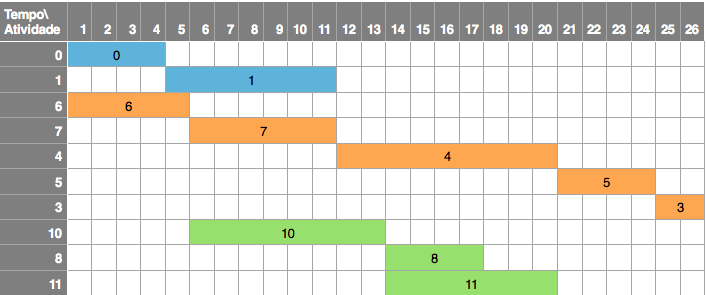
\includegraphics[width=\textwidth]{gant1}
\end{center}


\subsection{Questão 5}
Com base no diagrama previamente apresentado, e escolhendo a tarefa sete do caminho crítico, verifica-se que a mesma deverá ser iniciada 5 unidades de tempo após o início do projeto, uma vez que apresenta a tarefa 6 como precedente e esta só termina no instante de tempo 5. 
O mesmo pode ser verificado no ficheiro de output do LPSolve, através do valor da variável $t_7$ que toma o valor de 5 unidades de tempo.

\subsection{Questão 6}

Passemos agora à análise de uma tarefa que não faz parte do caminho crítico. Por exemplo, tomando como objeto de estudo a tarefa zero que não possui nenhuma precedência, mas faz parte da precedência da tarefa um.
A tarefa zero, uma vez que não possui nenhuma precedência, pode ser iniciada, no mínimo, no instante inicial do projeto; como a tarefa zero tem uma duração de 4 unidades de tempo e a tarefa um uma duração de 6 unidades de tempo, a tarefa zero poderá ser iniciada, no máximo, 11 unidades de tempo antes do fim do projeto, ou seja, no instante de tempo 15 e, ainda assim, não causar atrasos no projeto que tem uma duração de 26 unidades de tempo.
Essa janela de tempo $[0,15]$ é trivialmente verificada no diagrama de Gantt abaixo representado: 
\begin{center}
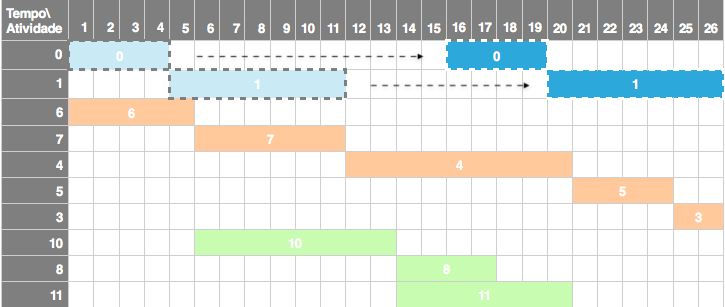
\includegraphics[width=\textwidth]{gant4}
\end{center}

%%%%%%%%%%%%%%%%%%%%%%%%%%%%%%%%%%%%%%%%%%%%%%%%%%%%%%%%%%%%%%
\section{Parte III}
 %%%%%%%%%%%%%%%%%%%%%%%%%%%%%%%%%%%%%%%%%%%%%%%%%%%%%%%%%%%%%%
\subsection{Questão 1}

Nesta parte, é associado a cada atividade um custo monetário de execução, e a possibilidade de reduzir a duração de cada uma destas.
No entanto, o número de reduções da duração de uma atividade tem um limite e um custo por unidade de tempo associado. O objetivo é reduzir o tempo de execução encontrado na \textbf{Parte I} (que também coincide com a \textbf{Parte II}) do projeto por 3 unidades temporais, minimizando o custo suplementar causado pelas reduções.
Como variáveis de decisão, temos $r_{[atividade]}$ que representa o número de reduções efetuadas na duração da atividade correspondente.
A função objetivo será constituída pela soma dos valores de custo normal de cada atividade, com o resultado do produto entre o valor de cada redução e o número de reduções feitas. Esta função objetivo representa o custo total do projeto (cujo objetivo é minimizar) e é:
\begin{Verbatim}[frame=single]
min:400+100r0+1000+300r1+300+100r3+2000+400r4+1000+800r5+800+90r6+900+600+100r8+
1600+500r10+1400+300r11+r7+ri;
\end{Verbatim}

que pode ser simplificada como:

\begin{Verbatim}[frame=single]
min: 10000+100r0+300r1+100r3+400r4+800r5+90r6+100r8+500r10+300r11+r7+ri;
\end{Verbatim}

Neste modelo, a primeira restrição diz respeito à variável $t_f$ e representa o tempo mínimo pretendido para o projeto, que será menor ou igual a 23. As restantes restrições dizem respeito ao limite de reduções permitidas em cada atividade. Por fim, o tempo de início de uma dada atividade deverá ser maior ou igual do que a duração da atividade anterior, somando a diferença entre o tempo normal da atividade e número de unidades temporais de redução da mesma. 
Este modelo é uma variação do modelo da \textbf{Parte II}, incluindo apenas as possíveis reduções da duração de cada atividade. Contudo, é fácil verificar que dadas as relações de precedência e o conceito de caminho crítico, tais reduções irão afetar a duração do projeto de uma forma dinâmica.

\subsection{Questão 2}

Input do LPSolve:

\begin{Verbatim}[frame=single]
/* Objective function */
min: 10000+100r0+300r1+100r3+400r4+800r5+90r6+100r8+500r10+300r11+r7+ri;

/* Restrictions - Precedências Temporais + Reduções (c/ Custo Associado) */

//Factor de Optimização
tf<=23;

//Limite superior das reduções
ri=0;
r7=0;
r0<=1;
r1<=2;
r3<=1;
r4<=3;
r5<=1;
r6<=2;
r8<=1;
r10<=1;
r11<=2;

//precedências temporais
t0>=0;
t1>=4-r0+t0;
t3>=6-r1+t1;
t3>=9-r4+t4;
t3>=4-r5+t5;
t4>=4-r0+t0;
t4>=6-r7+t7;
t5>=9-r4+t4;
t5>=4-r8+t8;
t6>=0;
t7>=5-r6+t6;
t8>=6-r7+t7;
t8>=8-r10+t10;
t10>=5-r6+t6;
t11>=8-r10+t10;
tf>=2-r3+t3;
tf>=4-r5+t5;
tf>=4-r8+t8;
tf>=7-r11+t11;

\end{Verbatim}

\subsection{Questão 3}
Output do LPSolve:
\begin{Verbatim}[frame=single]
Variables	result
		 10280
r0		 0
r1		 0
r3		 1
r4		 0
r5		 0
r6		 2
r8		 0
r10		0
r11		0
r7		 0
ri		 0
tf		23
t0		 0
t1		16
t3		22
t4		 9
t5		18
t7		 3
t8		11
t6		 0
t10		3
t11	       16
\end{Verbatim}


\subsection{Questão 4}

Resolvido o problema apresentado e obtido o output com auxilio do LPSolve, verifica-se que a duração da \textit{atividade 3} deve ser reduzida por uma unidade de tempo, com um custo associado de 100 unidades monetárias (UM), e que a duração da \textit{atividade 6} deve ser reduzida por 2 unidades de tempo, com um custo de 180 U.M.


\begin{center}
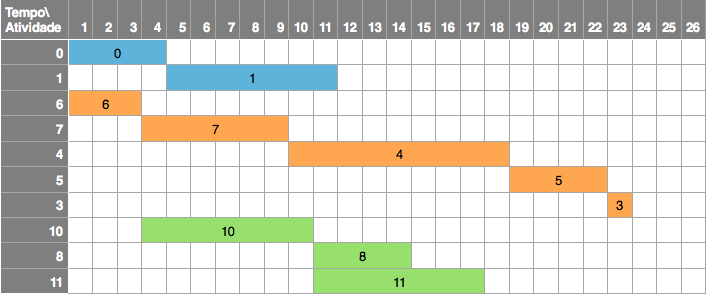
\includegraphics[width=\textwidth]{gant2}
\end{center}



Somando os valores dos custos normais de cada atividade com o custo das reduções, temos:	
		$$10000 + 100*1 + 90*2 = 10280 \hspace {0.2cm}U.M. $$
Que é igual ao resultado da função objetivo apresentado pelo output do programa, e portanto, mostrando que o custo da solução ótima está correto.



%%%%%%%%%%%%%%%%%%%%%%%%%%%%%%%%%%%%%%%%%%%%%%%%%%%%%%%%%%%%%%
\section{Parte IV}
%%%%%%%%%%%%%%%%%%%%%%%%%%%%%%%%%%%%%%%%%%%%%%%%%%%%%%%%%%%%%%
	\vspace{20pt}
	\begin{center}
		\begin{tabular}{|c|c|c|c|c|c|c|c|c|c|}\hline
			$x$&19&20&21&22&23&24&25&26 \\ \hline
			$f_(x)$&10000&10090&10180&10280&10680&11080&11480&12280 \\ \hline
	\end{tabular}
	\end{center}
	\vspace{20pt}
	Nesta parte, foi proposto que se criasse um gráfico que permitisse identificar os diferentes custos em função das possibilidades de tempo de execução do projeto. Para isso, foi criada a tabela acima, que tem o registo das sucessivas execuções do modelo anterior (\textbf{Parte III}). Em cada execução é alterada a restrição respeitante à variável $t_f$, alterando-se, assim, o tempo de execução do projeto e obtendo-se, consequentemente, os custos mínimos associados a cada execução.
	Analisando o gráfico abaixo, é possível concluir que o tempo normal para a conclusão do projeto é de 26 unidades de tempo (UT), apresentando o custo mais baixo de 10.000 UM. O tempo mínimo possível para a conclusão do projeto é 19 UT. apresentando um custo máximo de 12.280 UM. 
	O gráfico permite, ainda, ter uma visão global do comportamento das diferentes durações do projeto face aos respetivos custos.
	
	\begin{center}
		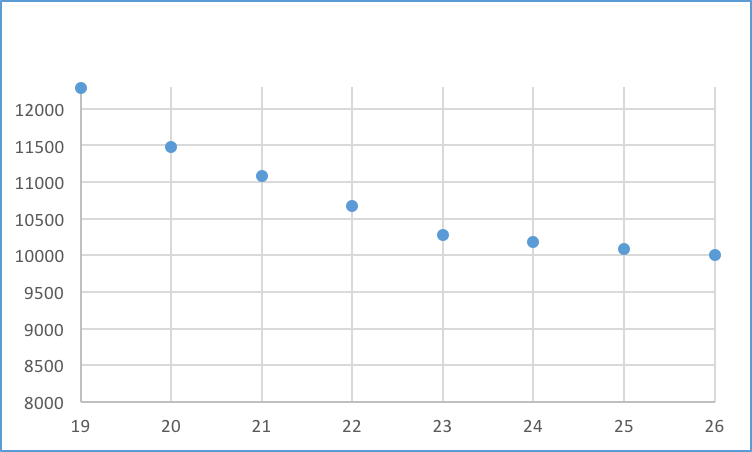
\includegraphics[width=\textwidth]{grafico.png}
	\end{center}
%%%%%%%%%%%%%%%%%%%%%%%%%%%%%%%%%%%%%%%%%%%%%%%%%%%%%%%%%%%%%%
\section{Parte V}
%%%%%%%%%%%%%%%%%%%%%%%%%%%%%%%%%%%%%%%%%%%%%%%%%%%%%%%%%%%%%%
\subsection{Questão 1}
O problema apresentado é uma variação daquele presente na \textbf{Parte III}, mas com um conjunto maior de reduções e custos, que resulta de aproximação linear de custo e reduções não-linear. Neste caso, cada atividade tem um custo de redução $c_1$ com um número máximo de reduções associado. Tem também um custo de redução $c_2$ e correspondente número máximo de reduções. Este último tipo de redução só pode ser aplicado se o número máximo de reduções $c_1$ for atingido. 
De facto, esta garantia é dada pela restrição:
$$c_1 \geq c_2$$ 
No entanto, qualquer que seja a atividade do projeto, os custos de reduções por UT associados às reduções do tipo $c_1$ são sempre inferiores aos do tipo $c_2$. Como tal, a restrição não é necessária, já que a função objetivo é minimizante. 
São ainda usadas as variáveis que representam o tempo de início de uma atividade: 
$$r_{[atividade] [tipo]}$$ 
Estas representam o número de reduções de cada atividade e o tipo correspondente. O número máximo de reduções das atividades, no projeto, é de 4 UT, tendo em conta  o custo suplementar de cada redução.
A função objetivo será semelhante à usada na \textbf{Parte III}, com o somatório dos valores de custo normal de cada atividade e o produto de cada variável $r_{[atividade] [tipo]}$ com o custo suplementar correspondente. Mais uma vez, esta função representa o custo a minimizar:
\begin{Verbatim}[frame=single]		
	min:400+100r01+200r02+1000+300r11+600r12+300+100r31+200r32+2000+400r41+
	800r42+1000+800r51+1600r52+800+90r61+180r62+900+600+100r81+200r82+1600+
	500r101+1000r102+1400+300r111+600r112;
\end{Verbatim}

Em relação ao modelo da \textbf{Parte III}, as restrições foram alteradas de forma a acomodar a nova representação das reduções. Cada variável $r_{[atividade] [tipo]}$ é limitada pelo seu respetivo número máximo de reduções, e na representação das precedências temporais subtrai-se o número de reduções possíveis de cada tipo, ao tempo de início da atividade precedente, somado com a duração da atividade precedente. Por fim, estará presente que $t_f \leqslant  22$, representando a redução de 4 UT à duração do projeto.
É de notar que poderiam ser utilizadas aproximações mais precisas, de forma sistemática, aumentado o número de variáveis de decisão, para a função não-linear que representa o custo da redução. Para tal, bastaria apenas repetir o processo apresentado aqui em relação ao modelo base (apresentado na \textbf{Parte III}).


	
\subsection{Questão 2}
\begin{Verbatim}[frame=single]
/*Função Objetivo */
min:400+100r01+200r02+1000+300r11+600r12+300+100r31+200r32+2000+400r41+
800r42+1000+800r51+1600r52+800+90r61+180r62+900+600+100r81+200r82+1600+
500r101+1000r102+1400+300r111+600r112;

/* Restrições - precedências Temporais + Reduções (c/ Custo Associado) */

//factor de optimização
tf<=22;

//Limite superior das reduções
ri=0;
r71=0;
r72=0;

r01<=0.5;
r11<=1;
r31<=0.5;
r41<=1;
r51<=0.5;
r61<=1;
r81<=0.5;
r101<=0.5;
r111<=1;

r02<=0.5;
r12<=1;
r32<=0.5;
r42<=2;
r52<=0.5;
r62<=1;
r82<=0.5;
r102<=0.5;
r112<=1;

//precedências temporais
t0>=0;
t1>=4-r01-r02+t0;
t3>=6-r11-r12+t1;
t3>=9-r41-r42+t4;
t3>=4-r51-r52+t5;
t4>=4-r01-r02+t0;
t4>=6-r71-r72+t7;
t5>=9-r41-r42+t4;
t5>=4-r81-r82+t8;
t6>=0;
t7>=5-r61-r62+t6;
t8>=6-r71-r72+t7;
t8>=8-r101-r102+t10;
t10>=5-r61-r62+t6;
t11>=8-r101-r102+t10;
tf>=2-r31-r32+t3;
tf>=4-r51-r52+t5;
tf>=4-r81-r82+t8;
tf>=7-r111-r112+t11;
\end{Verbatim}

\subsection{Questão 3}
Output do LPSolve:
\begin{Verbatim}[frame=single]
Variables	result
		 10820
r01		0
r02		0
r11		0
r12		0
r31	        0,5
r32		0,5
r41		1
r42		0
r51		0
r52		0
r61		1
r62		1
r81		0
r82		0
r101	       0
r102	       0
r111	       0
r112	       0
tf		22
ri	         0
r71		0
r72		0
t0		 0
t1		 4
t3		21
t4		 9
t5		17
t7		 3
t8		11
t6		 0
t10		3
t11	       11
\end{Verbatim}

\subsection{Questão 4}

Resolvido o problema apresentado e obtido o output com auxílio do LPSolve, verifica-se que a duração da \textit{atividade 3} deve ser reduzida por 0.5 UT a custo $c_1$ e 0.5 UT a custo $c_2$, com um custo total de 150 UM. A duração da \textit{atividade 4} deve ser reduzida por 1 UT a custo $c_1$, com um custo total 400, e a duração da \textit{atividade 6} deve ser reduzida por 1 UT a custo $c_1$ e 1 UT a custo $c_2$, com um custo total de 270 UM.

\begin{center}
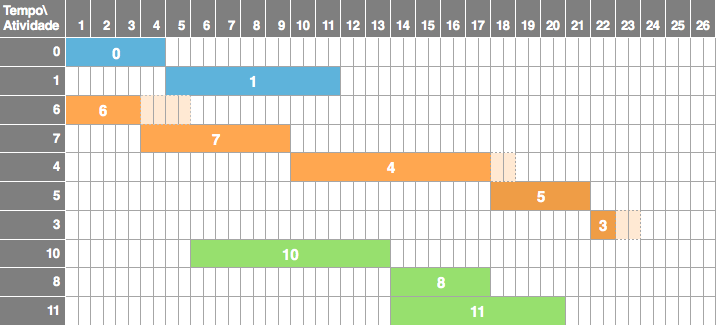
\includegraphics[width=\textwidth]{gant3}
\end{center}


Somando os valores dos custos normais de cada atividade com o custo das reduções, temos $$10000 +100*0.5+200*0.5+400*1+90*1+180*1 = 10820 \hspace{0.2cm} UM $$ que é igual ao resultado da função objetivo apresentado pelo output do programa.
%%%%%%%%%%%%%%%%%%%%%%%%%%%%%%%%%%%%%%%%%%%%%%%%%%%%%%%%%%%%%%
\section{Conclusão % e Trabalho Futuro
}
%%%%%%%%%%%%%%%%%%%%%%%%%%%%%%%%%%%%%%%%%%%%%%%%%%%%%%%%%%%%%%
Este trabalho favoreceu a aplicação prática de conhecimentos teóricos de programação linear. Permitiu desenvolver e refinar os métodos de abordagem de problemas relativamente complexos de modelação de sistemas lineares.
Relativamente à resolução do trabalho, as maiores dificuldades surgiram inicialmente na modelação do problema da \textbf{Parte III}, ao nível particular da determinação das restrições de precedência temporal do mesmo. Contudo, o estudo de outros exemplos práticos mostrou-se uma mais valia para superar esta dificuldade.
Este projeto permitiu também ao grupo a familiarização com a aplicação LPSolve, uma ferramenta poderosa que permite calcular a forma mais eficiente na resolução de problemas de programação linear. 






\end{document}
